%!TEX root = thesis.tex

\chapter{Introduction}
\par
Creating detailed virtual worlds can be a tedious task for artists. Indeed, modelling terrain, vegetation, water streams, rivers, water reserves, soil, rocks, buildings and road networks for large virtual worlds "by hand" can be extremely burdensome. This is especially true when realism is a key requirement. The increase in size and complexity of these virtual worlds mirror that of the processing capabilities of computing hardware. As a consequence, the task is only getting worse.\\

A popular technique to overcome the burden of repetitive tasks is to have them automated. This involves generating algorithms which, given a set of input parameters, generate the required content automatically. This is called \textit{procedural content generation} and has already been successfully applied in different areas of computer graphics including: the generation of non-repetitive textures \cite{Efros1999,Liang2001,Wei2009}, modelling plants \cite{Boudon2012,Fourcaud2008,Guo2011,Lewis1999}, generating terrains \cite{Smelik2009,Gain2009,Doran2010}, generating river networks \cite{Derzapf2011,Emilien} and generating city landscapes \cite{Gain,Kelly2007,Parish2001} (figure \ref{Example of procedurally generated content}) \\
A common difficulty with these methods, however, is finding the appropriate input parameters for the procedural algorithms. The correlation between the parameters and the resulting content is often unintuitive and, as a consequence, often comes down to iterative trial-and-errors until a "close enough" result is found. To overcome this, interactive techniques are often used in an attempt to make generating the input parameters more intuitive. These range from simple paint tools such as lassos and brushes \cite{Emilien} to sketch-based recognition algorithms \cite{Gain2009}. \\

\begin{figure}[h]
  \centering
	\label{Example of procedurally generated content}
	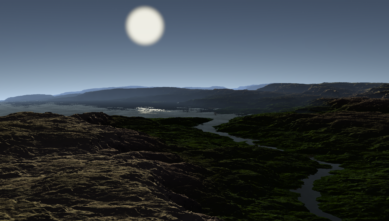
\includegraphics[natwidth=389,natheight=222]{procedural_generated_river.png}
	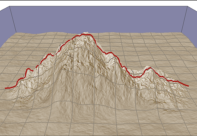
\includegraphics[natwidth=197,natheight=136]{procedural_generated_terrain.png}
	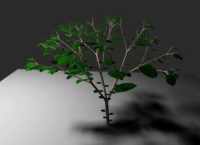
\includegraphics[natwidth=200,natheight=145]{procedural_generated_plant.png}
	\caption{Example of procedurally generated content. From top to bottom, left to right: Procedurally generated river stream \cite{Derzapf2011}, procedurally generated terrain through sketching \cite{Gain2009}, procedurally generated plant \cite{Soler2001}}
\end{figure}

The intent of this thesis is to develop procedural algorithms to automate the generation of virtual rural worlds. The input parameters for the procedural algorithms must be interactive and/or self-explanatory. 

\newpage
\section{Research Goals}

The research goals for this project are as follows:
\begin{itemize}
\item Develop procedural methods to automate the generation of realistic virtual rural worlds.
\item Provide intuitive and smart controls.
\item When possible, make interactions real-time.
\end{itemize}

One of the most important aspect of rural landscapes is vegetation. As such, our \textit{first goal} must strongly focus on the insertion of plants. The automation provided should not limit user control and the flexibility of the system. For example, it must be possible to generate worlds with varying elevations, river networks, water sources and vegetation.\\

For the \textit{second goal}, lots of thought must be put into making all user oriented controls intuitive. To do so, it will be important to research the pros and cons of other graphical applications in terms of control. If need be, multiple prototype controls should be developed in an attempt to find the best suited.\\

Maintaining a continuous feedback loop between user action and corresponding reaction is extremely important for both user-friendliness and to optimize usage. In an attempt to meet our \textit{third goal} therefore, efficient algorithms must be developed in order to keep there time complexity to a minimum. When suited, these algorithms should be developed to run on the GPU. \\

\section{Contributions}
\todo{State contributions of this thesis}

\section{Structure}
\todo{Outline structure of the thesis}
